\documentclass{article}

\usepackage{geometry}
\usepackage{amsmath}
\usepackage{graphicx}
\usepackage{listings}
\usepackage{hyperref}
\usepackage{multicol}
\usepackage{fancyhdr}
\pagestyle{fancy}
\hypersetup{ colorlinks=true, linkcolor=black, filecolor=magenta, urlcolor=cyan}
\geometry{ a4paper, total={170mm,257mm}, top=20mm, right=20mm, bottom=20mm, left=20mm}
\setlength{\parindent}{0pt}
\setlength{\parskip}{1em}
\renewcommand{\headrulewidth}{0pt}
\lhead{Competitive Programming - Arkavidia V}
\fancyfoot[CE,CO]{\thepage}

\begin{document}

\begin{center}
    \section*{E. Ekspedisi ke Dimensi 8}

    \begin{tabular}{ | c c | }
        \hline
        Batas Waktu  & 10s \\
        Batas Memori & 256MB \\
        \hline
    \end{tabular}
\end{center}

\subsection*{Deskripsi}

Arvy sudah belajar konsep array (larik) pada programming.
Ia tertarik menghitung jumlah dari subarray.
Jumlah dari subarray ($i, j$) adalah jumlah dari elemen $A_i, A_{i+1}, \dots, A_{j-1}, A_j$.
Namun ia tertantang untuk berekspedisi ke dimensi lebih tinggi.
Pada 2 dimensi, subarray berbentuk persegi panjang atau matriks.
Pada 3 dimensi, subarray berbentuk balok.
Perhitungan ini dapat digeneralisasikan hingga dimensi lebih tinggi lagi.

Pada dimensi $D$, kita menandai tiap elemen dengan indeks berupa vektor yang terdiri dari $D$ elemen.
Permasalahan subarray dengan batas vektor $l$ dan $r$ dapat digeneralisasikan menjadi jumlah dari semua elemen yang memiliki vektor indeks $A$ sehingga $l_i \leq A_i \leq r_i$.

\subsection*{Format Masukan}

Baris pertama terdiri dari satu bilangan bulat positif $T$ ($1 \leq T \leq 5$), menyatakan banyaknya kasus uji.

Tiap kasus uji diawali dengan bilangan $D$ ($1 \leq D \leq 8$), menyatakan dimensi dari array.
Baris selanjutnya terdiri dari $D$ bilangan $L$ dipisahkan oleh spasi, dengan $D_i$ menyatakan ukuran array di dimensi ke-$i$.
Baris selanjutnya terdiri dari $1 \leq \prod_{i=1}^{D}{D_i} \leq 100.000$ bilangan, menyatakan elemen array ($|elemen| \leq 100.000$), jika diurutkan berdasarkan indeksnya secara leksikografis.

Baris selanjutnya terdiri dari sebuah bilangan $Q$ ($1 \leq Q \leq 100$) menyatakan jumlah pertanyaan.
Setiap pertanyaan ditulis dalam 2 baris, berupa vektor $l$ pada baris pertama dan $r$ pada baris kedua. Vektor $l$ dan $r$ memiliki $D$ elemen, dan masing-masing elemen ($1 \leq l_i \leq r_i, \leq L_i$) dipisahkan oleh spasi.

Catatan: vektor indeks $A$ dianggap kurang dari $B$ secara leksikografis bila ada $i$ sehingga $A_i < B_i$ dan untuk tiap $j$ yang memenuhi $0 \leq j < i$, $A_j = B_j$.

\subsection*{Format Keluaran}

Untuk tiap kasus uji, tuliskan $Q$ baris, yakni jawaban dari masing-masing pertanyaan.

\pagebreak

\begin{multicols}{2}
\subsection*{Contoh Masukan}
\begin{lstlisting}
2
1
5
1 2 3 4 5
2
1
3
2
5
2
4 5
1 2 7 5 4 -10 5 -1 -3 2 3 4 4 -8 11 -3 3 7 -1 9
3
1 2
2 2
3 3
4 5
3 2
4 3
\end{lstlisting}
\columnbreak
\subsection*{Contoh Keluaran}
\begin{lstlisting}
6
14
7
22
18
\end{lstlisting}
\vfill
\null
\end{multicols}

\subsection*{Penjelasan}
Pada kasus uji pertama, kita memiliki array 1 dimensi, sehinnga jawaban tiap pertanyaan adalah:
\begin{itemize}
    \item Dari indeks (1) sampai (3), $1 + 2 + 3 = 6$
    \item Dari indeks (2) sampai (5), $2 + 3 + 4 + 5 = 14$
\end{itemize}

Pada kasus uji kedua, kita memiliki array 2 dimensi yang dapat digambarkan sebagai berikut (indeks (1, 1) ada di kiri atas):

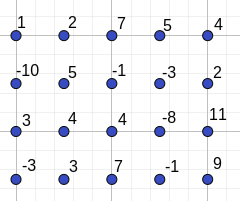
\includegraphics[width=150px]{sample-2}

\begin{itemize}
    \item Dari indeks (1, 2) sampai (2, 2), $2 + 5 = 7$
    \item Dari indeks (3, 3) sampai (4, 5), $4 - 8 + 11 + 7 - 1 + 9 = 22$
    \item Dari indeks (3, 2) sampai (4, 3), $4 + 4 + 3 + 7 = 18$
\end{itemize}

\pagebreak

\end{document}